\subsection{Prof. Dr. Arvid Kappas}


\textbf{Main Research Interests}\\[-0.25cm]
\begin{enumerate}
\item[$\bullet$]	Emotions, specifically Expressive Behavior and Psychophysiological Responses in Social Context
\item[$\bullet$]	Perception of Facial Expressions of Emotions
\item[$\bullet$]	Interaction with Robots and Avatars
\item[$\bullet$]	The Impact of Information Processing (Appraisals) on Human Emotions
\item[$\bullet$]	Communication of Emotions over the Internet.
\end{enumerate}


\vspace{0.6cm}
\textbf{Research Activities}\\[-0.25cm]

Much of Arvid Kappas' current research centers around the role of implicit processing in social context effects of facial behavior. This research uses a variety of paradigms, including inducing affective behavioral responses, assessed using facial electromyography (EMG) as well as Implicit Association Tasks and a modified version of the Affective Simon Task. The goal of these experiments is to understand the processes underlying the behavioral phenomena first demonstrated by Hess, Banse, and Kappas (1995). The experimental work is linked to the PhD thesis of Dennis K�ster as well as with the preparation of a DFG grant proposal. Early results have already been presented at international conferences and manuscripts are currently being prepared to be submitted. A transdisciplinary research project (with Olk and M�ller, IUB) investigates how different groups of people perceive press photography, how they interpret the visuals and how they react to them. The project is unique as it combines for the first time the methods of eye tracking (perception analysis), iconology (meaning interpretation) and psychophysiological measurement (emotional reaction). Collaborative research is ongoing with Eva Krumhuber and Antony Manstead (Cardiff University, UK) on the perception of facial behavior. In this latter line of research synthetic faces are used to create dynamic stimuli to understand the role of temporal aspects of facial displays in person and expression perception. Further research is ongoing with John Charlton (Bolton University, UK) on anger while driving and computing. Furthermore, Arvid Kappas is in the early stages of collaboration with Thalia Wheatley (Dartmouth College) on the perception of human and artificial movements and Paul Whalen (Dartmouth College) on the role of specific components of smiling behavior.
\\
\begin{}
  \begin{center}
    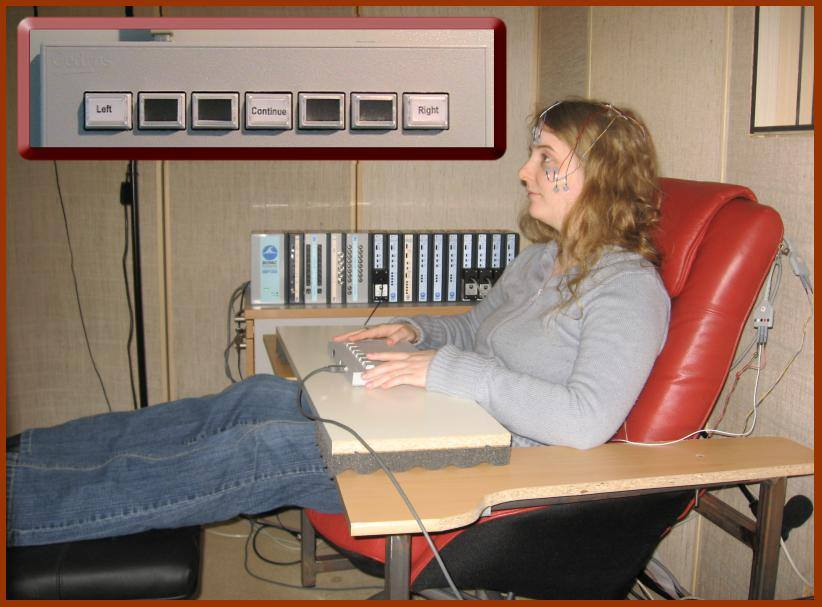
\includegraphics[width=0.65\textwidth]{./Psy/Kappas1.jpg}
    
    \caption{\itshape Facial activity is recorded using electromyography (EMG) while participant is watching emotional video clips. Inset shows the response box used to collect the responses of the participant. The experiment takes place in a sound-isolated box. Films are projected through a window from the neighboring control room.}%\label{fig:profxxx}
   \end{center}
\end{figure}

\begin{}
  \begin{center}
    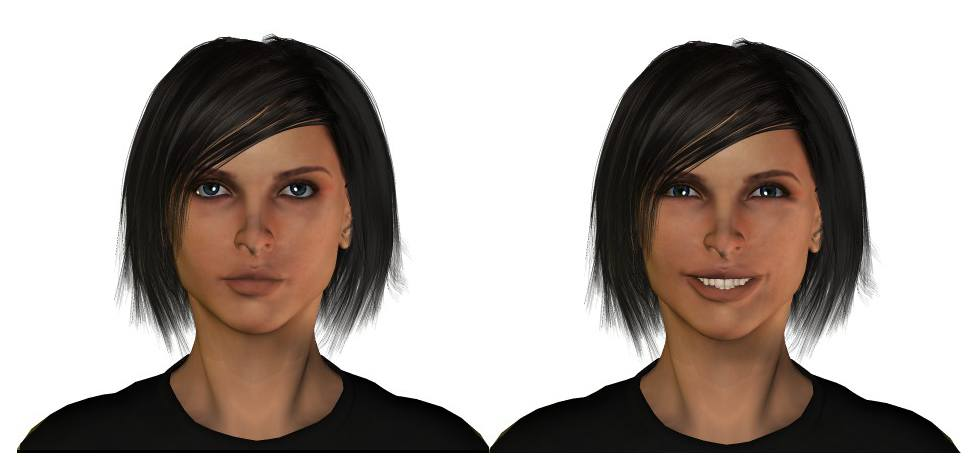
\includegraphics[width=0.8\textwidth]{./Psy/Kappas2.jpg}
    
    \caption{\itshape These faces were created using POSER 6 software (e frontier) and are used to study, for example, the role of temporal aspects of facial displays in person and expression perception.}%\label{fig:profxxx}
   \end{center}
\end{figure}

\vspace{0.6cm}


\vspace{0.6cm}
\textbf{Other Professional Activities}\\[-0.25cm]
\begin{enumerate}
\item[$\bullet$] Associate editor of Biological Psychology (Elsevier)
\item[$\bullet$] Member of editorial board of Journal of Nonverbal Behavior (Springer)
\item[$\bullet$] Editorial board of advisors of Cognition and Emotion (Taylor \& Francis)
\item[$\bullet$] Editorial consultant for British Journal of Social Psychology (British Psychological Society)
\item[$\bullet$] Board of Advisors The Centre for the Study of Emotion, University of Portsmouth
\item[$\bullet$] Reviews for further numerous journals as well as books.
\item[$\bullet$] Active member of several international scientific organizations; Charter member of the Association for Psychological Science, Fellow of the International Organization for Psychophysiology.
\end{enumerate}


\vspace{0.6cm}
\textbf{PhD-Students}\\[-0.25cm]

Dennis K\"{u}ster\newline
\textit{Processes of Implicit and Explicit Sociality in Regulation of Emotional Displays}\\[-0.15cm]

